\documentclass[accentcolor=tud1c, paper=a4, colorback]{tudreport}
\usepackage[ngerman]{babel}
\usepackage[utf8]{inputenc}

\usepackage[german]{todonotes}
\usepackage{amsmath, imakeidx, graphicx, hyperref}

%opening
\title{Bedienungsanleitung Flugsimulator}
\subtitle{BP-Team 19}
\subsubtitle{Wintersemester 17/18}
\makeindex

\newcommand{\ind}[1]{#1\index{#1}}
\graphicspath{ {img/} }

\begin{document}
	\maketitle
	\tableofcontents
	
	\todototoc
	\listoftodos

	\chapter{Präambel}
	\todo[inline]{basic Infos einfügen}
	\todo[inline]{Präambel zu geschlechtergerechten Sprache}
	
	\chapter{Einführung}
	
	\section{Aufbau der Software}
	Aufgrund der Netzwerktopologie ist die Software nach dem sogenannten
	\ind{Client-Server-System}\footnote{\url{https://en.wikipedia.org/wiki/Client-server\_model}}
	aufgebaut.
	\begin{figure}[h]
		\centering
		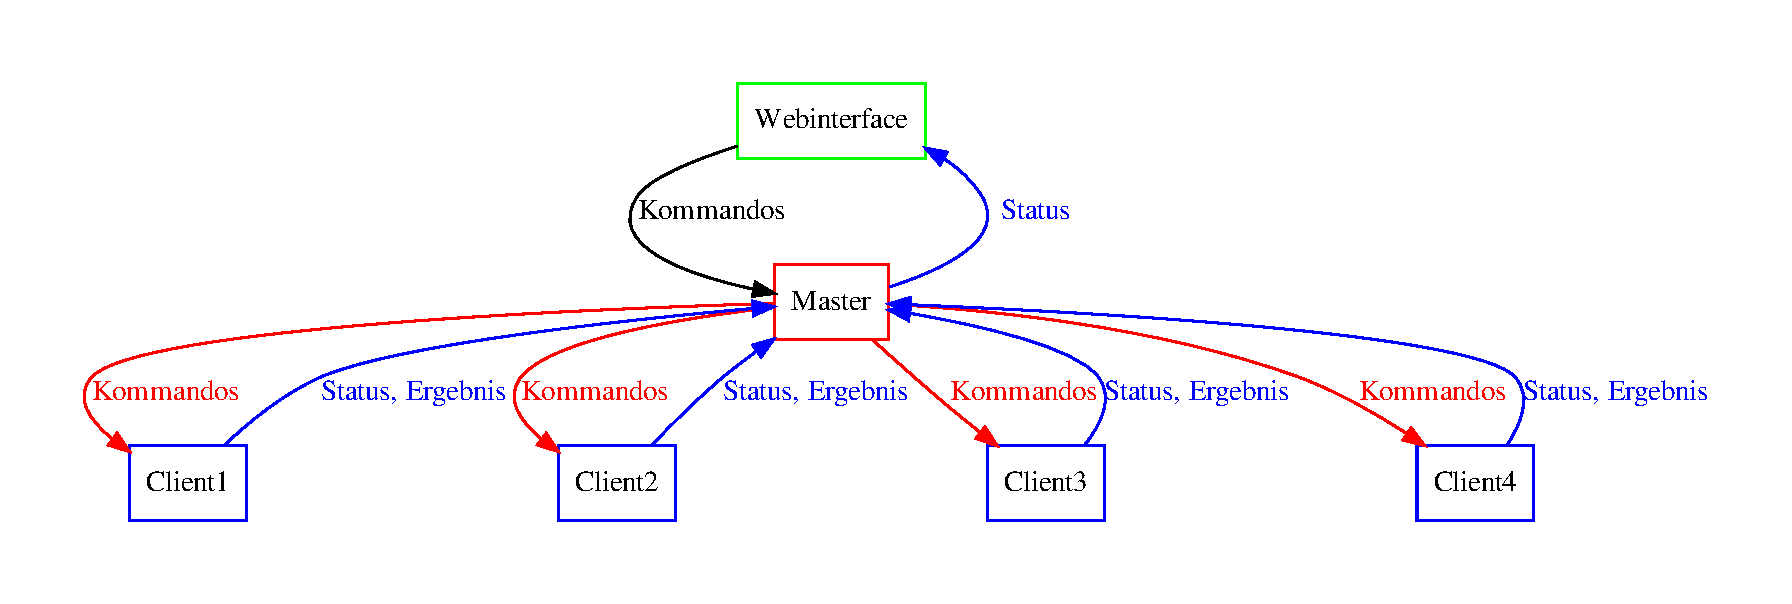
\includegraphics[width=\textwidth]{softwarelayout}
		\caption{Aufbau der Flugsimulatorsteuerung}
	\end{figure}
	\\
	Die Nutzer*innen kommunizieren über ein Webinterface mit dem Masterserver,
	welcher die Befehle dann an die einzelnen Clients weiterleitet.
	\\
	Die Serverkomponente ist in der Programmiersprache \ind{Python}\footnote{\url{https://www.python.org/}}
	in der aktuellen Version 3 geschrieben. Um die Menge an notwendigem Code möglichst
	klein zu halten, wurde auf möglichst verbreitete Frameworks zurückgegriffen.
	Beispielsweise wird das Webinterface auf Serverseite durch das Framework \ind{Django}\footnote{\url{https://www.djangoproject.com/}}
	realisiert, welches sich gerade unter Pythonentwickler*innen sich großer Beliebtheit erfreut.
	Eine Anleitung, wie die Software korrekt aufgesetzt wird, findet sich im Repository des
	Projekts\footnote{\url{https://github.com/bp-flugsimulator/server/blob/master/README.md}}.
	\\
	Die Clients werden ebenfalls von einer Python Software gesteuert. Diese braucht lokal keine Konfiguration,
	bis auf die Adresse des Masterservers. Dieser übernimmt dann die komplette Konfiguration und Steuerung.
	\section{Terminologie}
	Im folgenden werden die einzelnen Begriffe der Software erklärt. Dies dient vor allem dem Verständnis
	der weiteren Kapitel.
	
	\subsection{\ind{Master}}
	Der zentrale Steuerungsrechner, auf welchem der Webserver läuft. Zur Zeit ist das der \ind{Simcontrol} Rechner.
	Im Standardfall wird die Weboberfläche der Anwendung hier geöffnet, sollte sich der Rechner aber im 
	Institutsnetz befinden, so lässt sich die Ansteuerung und Programmierung des Simulators auch vom
	Arbeitsplatzrechner erledigen. Wichtig ist aber, dass der Master Server nicht direkt aus dem Internet
	ansprechbar ist, da von Seiten der Software bisher keinerlei Authentifizierung vorrausgesetzt wird.
	
	\subsection{\ind{Client}}
	\missingfigure{Bild der Software mit einem Client}
	Ein Client ist jeder Rechner außer dem Master, welcher als Teil des Flugsimulators Programme ausführen muss.
	Das kann zum Beispiel \ind{Vision} sein, wobei ein Client auch für mehrere Programme verantwortlich
	sein kann.
	
	\subsection{\ind{Program}}
	\todo[inline]{evt. die deutsche Bezeichnung verwenden}
	Ein Program ist in dieser Software ein zu startendes Programm auf dem entsprechenden Client, beispielsweise
	X-Plane. Beim Anlegen in der Software werden unter anderem der Pfad mit der ausführbaren Datei, die Argumente
	und die Umgebung abgefragt, welche dan zum Starten des Programms verwendet werden.
	\missingfigure{Bild der Software mit einem Program (inklusive Optionen)}
	
	\subsection{\ind{Files}}
	\missingfigure{Bild der Software mit einem File}
	Um verschiedene Plugins nutzen zu können ist es manchmal notwendig, dass bestimmte Dateien innerhalb der
	X-Plane Ordner vor dem Start verschoben werden. Dazu lassen sich für jeden Client beliebig viele 
	Files
	definieren, welche die zu verschiebende Datei und ihren Zielort definieren. In einem Script lässt sich
	dann festlegen zu welchem Zeitpunkt die Datei kopiert werden soll. Sollte eine Datei am Zielort existieren,
	welche den gleichen Name wie die zu kopierende Datei besitzt, so wird ein Backup erstellt, welches beim
	Herunterfahren wiederhergestellt wird.
	
	\subsection{\ind{Script}}
	Um den Vorgang eines Startes zu automatisieren steht kann der/die Nutzer*in ein sogenanntes Script erstellen.
	Ein Script ist eine Liste an Anweisungen bestehend aus Files und Programs, welche in der spezifizierten
	Reihenfolge abgearbeitet werden. Dabei wird die Beschreibungssprache 
	\ind{JSON}\footnote{\url{https://en.wikipedia.org/wiki/JSON}} verwendet. Eine Dokumentation dieser Sprache
	befindet sich im Anhang (\autoref{json-ref}).

	\chapter{Workflows}
	\todo[inline]{Standardworkflows a la Eine Node Hinzufügen}
	\section{Einen Client hinzufügen}
	Nach dem Starten des Webservers muss im Browser die Weboberfläche geöffnet werden.
	Arbeitet man auf dem \ind{Simcontrol} direkt, so findet sich diese unter
	\url{http://localhost:8000/slaves}. Ansonsten muss anstatt \texttt{localhost}
	die \ind{IP-Ardresse} des Masters verwendet werden.
	\\
	\missingfigure{Weboberfläche ohne konfigurierte Nodes}
	Über den \texttt{+} Knopf neben dem Client-Schriftzug auf der linken Seite
	lässt sich ein neuer Client anlegen. Dazu ist ein Name, die IP-Addresse und
	die MAC-Adresse des Clients notwendig. Diese lassen sich unter Windows
	mit dem Befehl \texttt{ipconfig} herausfinden. Der Name kann frei gewählt
	werden und dient nur der Wiedererkennung in der Oberfläche.
	\\
	Nach dem Anlegen erscheint der Client in der linken Spalte. Durch Auswählen erhält
	man eine Übersicht mit den Programmen und Dateien des Clients. Zudem stehen die
	Knöpfe \texttt{Start}, \texttt{Edit} und \texttt{Delete} zur Verfügung.
	Während die Letztgenannten relativ selbsterklärend seien sollten, startet der
	erste Knopf den Rechner über das Netzwerk. Sollte der Befehl erfolgreich
	versendet worden sein, so wird eine Benachrichtigung angezeigt.
	\chapter{Anhang}
	\section{Referenz der Scriptsprache}
	\label{json-ref}
	\todo[inline]{Referenz für die Scriptsprache}

	\clearpage
	\addcontentsline{toc}{chapter}{Index}
	\printindex


\end{document}
